\chapter{Neutrino physics}
\section{Neutrinos in the Standard Model of Particle Physics}
\label{sec:nuIntro}
Neutrinos are elementary particles, specifically neutral leptons, that, according to the \ac{SM} of Particle Physics, only interact via weak interactions.  
They were first postulated in 1930 by the Austrian physicist Wolfgang Pauli to describe the continuous energy spectrum of beta decay. 
Since only the electron and the recoiling nucleus were observed, the process seemed to violate energy and spin conservation; therefore, Pauli introduced a third, 
unseen spin-1/2 particle to carry away the missing energy and balance the angular momentum.

They were eventually confirmed experimentally in 1956 by Clyde Cowan and Frederick Reines during an experiment conducted at the Savannah River 
nuclear reactor in South Carolina. 
This experiment exploited inverse beta decay, in which the postulated particle -specifically an electron antineutrino ($\overline{\nu}_e$)- 
interacts with a proton to produce a neutron and a positron, as described by Eq. \ref{eq:inverse_beta_decay}.
\begin{equation}
    \label{eq:inverse_beta_decay}
    \overline{\nu}_e + p \rightarrow n + e^{+}
\end{equation}
In the experimental setup, antineutrinos produced by the reactor fission processes interacted with protons in the water of two target tanks, 
yielding a positron and a neutron. The positron quickly annihilated with an adjacent electron, producing two prompt gamma rays. 
Meanwhile, the neutron thermalized and subsequently captured by the cadmium nuclei of cadmium chloride (CdCl$_2$) dissolved in the water tanks.
As a consequence of this neutron capture, an additional gamma-ray signal was released. The detection of these three gamma-ray signals 
in delayed coincidence provided an unambiguous signature of the antineutrino interaction, definitively confirming the existence of 
both neutrinos and antineutrinos \cite{cowan1956nudetection}.

Within the framework of the \ac{SM}, neutrinos are described as neutral fermions that do not participate in strong or 
electromagnetic interactions: they are colour singlets and carry no electric charge. The \ac{LH} neutrino of each family is grouped with the corresponding charged lepton ($\ell = e, \mu, \tau$) into a weak-isospin doublet $L_\ell = (\nu_\ell, \ell)^T_\text{L}$.
% , which transforms as $(\mathbf{1}, \mathbf{2}, -\tfrac{1}{2})$ under the gauge group SU$(3)_\text{C} \times$ SU$(2)_\text{L} \times$ U$(1)_Y$. The electromagnetic group U$(1)_\text{EM}$ is not part of the original gauge group: it is the subgroup that survives electroweak symmetry breaking, with $Q = T_3 + Y$. 
No \ac{RH} neutrino field is present in the minimal \ac{SM}.

The SU$(2)_\text{L}$ gauge invariance fixes the form of the weak interactions between neutrinos and the gauge bosons; neutrinos taking part in these interactions are called \textit{active}. These interactions consist of \ac{CC} processes mediated by the $W^\pm$ bosons and \ac{NC} processes mediated by the $Z^0$ boson, described by the following Lagrangians:
\begin{equation}
    \label{eq:SM-neutrino-lagrangian}
    \begin{aligned}
        \mathcal{L}_\text{CC} &= - \frac{g}{\sqrt{2}} \sum_{\ell} \overline{\nu}_{\text{L},\ell} \gamma^\mu \ell_\text{L}^- W_\mu^+ + \text{h.c.} \\
        \mathcal{L}_\text{NC} &= - \frac{g}{2 \cos \theta_W} \sum_{\ell} \overline{\nu}_{\text{L},\ell} \gamma^\mu \nu_{\text{L},\ell} Z_\mu^0
    \end{aligned}
\end{equation}
where $g$ is the SU$(2)_\text{L}$ coupling constant and $\theta_W$ is the Weinberg weak mixing angle. 

Precision measurements of the invisible decay width of the $Z^0$ boson at LEP constrain the number of active neutrino families to $N_\nu = 2.9963 \pm 0.0074$~\cite{JanotJadach2020}, consistent with the three known generations of charged leptons\footnote{The measurement only counts active neutrinos lighter than $m_Z/2$; it does not exclude sterile neutrinos.}.

% --------------------------------------------------------
% ----------------- FLAVOUR OSCILLATIONS -----------------
% --------------------------------------------------------
\section{Flavour oscillations}

% --------------------------------------------------------
% ---------------- EXPERIMENTAL EVIDENCES ----------------
% --------------------------------------------------------
\subsection[Experimental evidence: the solar neutrinos problem]{Experimental evidence: the solar neutrino problem\footnotemark}
\label{subsec:oscillation-experiments}
\footnotetext{All of what is reported in this section is elaborated from \cite{neutrinosPDG}, unless otherwise specified.}
\begin{wrapfigure}{l}{0.53\textwidth}
    \centering
    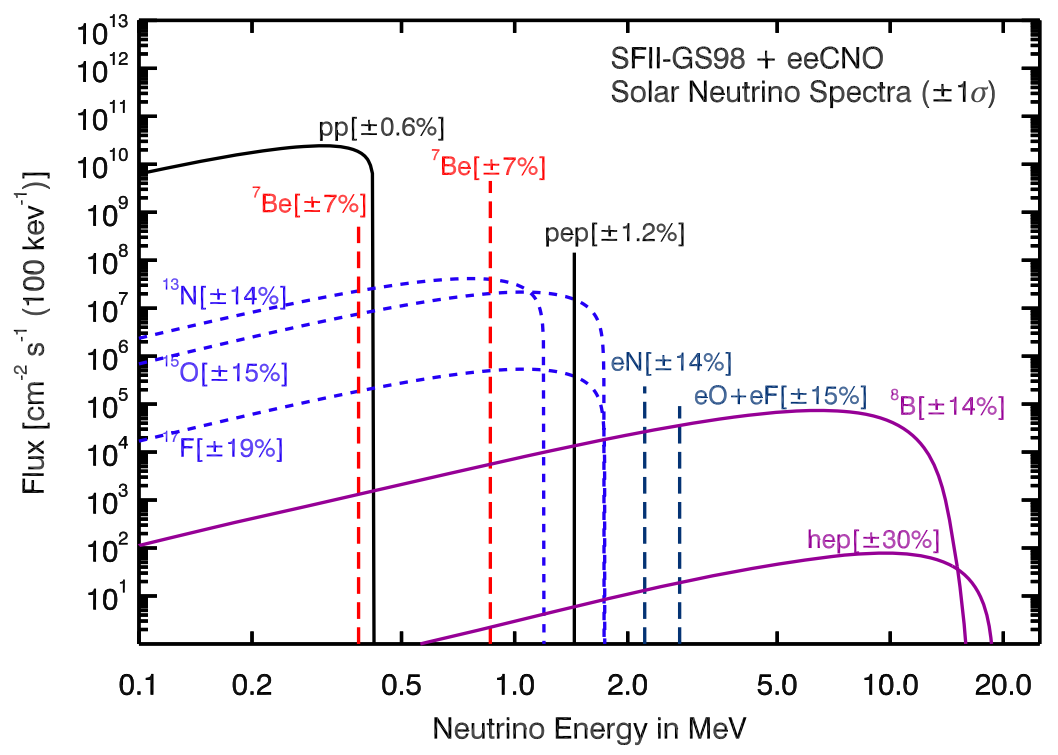
\includegraphics[width=\linewidth]{figures/neutrino-fluxes.png}
    \caption{Energy spectra of solar neutrino fluxes of different reaction processes. Plot taken from \cite{SunNuFluxes}.}
    \label{fig:neutrino-fluxes}
\end{wrapfigure}
Electron neutrinos are produced in the Sun in thermonuclear reactions that generate solar energy, namely \ac{pp} chains and \ac{CNO} cycles. Based on the \ac{SSM}, the total neutrino flux at Earth can be estimated from the solar luminosity. In the \ac{pp} chains four protons fuse into a ${}^4$He nucleus, $4p \to {}^4\text{He} + 2e^+ + 2\nu_e$, releasing $Q = 4M({}^1\text{H}) - M({}^4\text{He}) \sim 26.73$~MeV per chain; using atomic masses automatically includes the annihilation of the two positrons with electrons of the plasma. Only a small fraction of this energy, on average $\langle E_{2\nu}\rangle \simeq 0.59$~MeV, is carried away by the two neutrinos, while the rest heats the Sun and is eventually radiated as photons. Both \ac{pp} reactions and \ac{CNO} ones produce only $\nu_e$: the expected fluxes of the individual components, in the absence of oscillations, are shown in Figure~\ref{fig:neutrino-fluxes}.

Solar neutrinos have been detected since the late 1960s. The first solar neutrino experiment was performed underground in the Homestake gold mine in South Dakota, in order to prevent contamination from cosmic-ray induced reactions. It employed liquid tetrachloroethylene (C$_2$Cl$_4$) as the target, exploiting the \ac{CC} interaction $\nu_e + {}^{37}\text{Cl} \longrightarrow e^- + {}^{37}\text{Ar}$, whose threshold of $814$ keV makes it mainly sensitive to ${}^{7}$Be and ${}^{8}$B neutrinos. The measured rate was less than one third of the expected one, giving rise to the so-called \textit{solar neutrino problem}: the final result was $2.56 \pm 0.16 \pm 0.16 \text{ SNU}$~\footnote{SNU (solar neutrino unit) is a unit of event rate defined as $1 \text{ SNU} = 10^{-36}\text{ captures per second per target atom}$. The measured quantity is a capture rate, $R = \sum_i \Phi_i \sigma_i$, summed over the solar neutrino components $i$; converting it into a flux requires assuming the shape of the spectrum.}\cite{HomestakeResults}, to be compared with the \ac{SSM} prediction of $8.46^{+0.87}_{-0.88} \text{ SNU}$~\cite{SSMReference}.

Later, two radiochemical experiments, SAGE at the Baksan Neutrino Observatory and GALLEX (later followed by the Gallium Neutrino Observatory, GNO) at the Laboratori Nazionali del Gran Sasso (LNGS), exploited the gallium \ac{CC} interaction $\nu_e + {}^{71}\text{Ga} \longrightarrow e^- + {}^{71}\text{Ge}$, whose low threshold of $233$~keV makes it sensitive mainly to \ac{pp} neutrinos. SAGE reported $65.4^{+3.1+2.6}_{-3.0-2.8}$ SNU and GALLEX/GNO $69.3 \pm 4.1 \pm 3.6$ SNU, both in sharp contrast with the \ac{SSM} prediction of $127.9^{+8.1}_{-8.2}$ SNU for the same energy range, reinforcing the solar neutrino deficit puzzle.

From the 1990s, the Kamiokande and Super-Kamiokande water Cherenkov detectors pioneered real-time measurements of solar neutrino fluxes via elastic scattering ($\nu_\ell + e^- \longrightarrow \nu_\ell + e^-$). This signal is an indistinguishable mixture of \ac{CC} and \ac{NC} events, dominated by $\nu_e$ thanks to its larger cross-section. Sensitive mainly to ${}^8\text{B}$ neutrinos, Super-Kamiokande measured a flux of $(2.345 \pm 0.014 \pm 0.036) \times 10^{6} \text{ cm}^{-2}\text{s}^{-1}$~\cite{latestSUPERK}. This reveals a severe deficit compared to the theoretical \ac{SSM} prediction for ${}^8\text{B}$ neutrinos of $(5.46 \pm 0.66) \times 10^{6} \text{ cm}^{-2}\text{s}^{-1}$.

Finally, the Sudbury Neutrino Observatory (SNO) provided the model-independent proof that solar $\nu_e$ change flavour, using $1000$~t of heavy water ($\text{D}_2\text{O}$). Deuterium allowed SNO to measure separately the \ac{CC} interaction $\nu_e + d \to e^- + p + p$, sensitive only to $\nu_e$, and the \ac{NC} interaction $\nu_\ell + d \to  nu_\ell + p + n$, sensitive to all active flavours with equal cross-sections. The \ac{NC} channel measured a total active flux $\Phi_\text{SNO}^\text{NC} = (5.09 \pm 0.44  pm 0.46) \times 10^{6}~\text{cm}^{-2}\, \text{s}^{-1}$~\cite{SNO2002-results}, in agreement with the \ac{SSM} prediction, while the \ac{CC} channel gave $\Phi_\text{SNO}^\text{CC} = (1.76 \pm 0.05 \pm 0.09) \times 10^{6}~\text{cm}^{-2}\,\text{s}^{-1}$~\cite{SNO2002-results}. The ratio $\Phi^\text{CC}_\text{SNO}/\Phi^\text{NC}_\text{SNO}  simeq 0.35$ shows that about two thirds of the $\nu_e$ produced in the solar core reach the Earth as $\nu_\mu$ or $\nu_\tau$. The first conclusive evidence for neutrino oscillations had been obtained in 1998 by Super-Kamiokande with atmospheric neutrinos, through the up-down asymmetry of the $\nu_\mu$ flux~\cite{SuperK1998}.

The different deficit ratios observed by radiochemical experiments (Homestake, SAGE, GALLEX/GNO) and water Cherenkov detectors (Super-Kamiokande, SNO) arise because each experiment probes a different part of the solar neutrino energy spectrum, over which the $\nu_e$ survival probability varies. In the standard picture, this energy dependence results from the transition between vacuum-dominated oscillations at low energies and matter-enhanced conversion inside the Sun at high energies. The following two sections outline these two regimes, starting from the simpler case of oscillations in vacuum, whose formalism is also the basis for including matter effects.


% ----------------------------------------------------------
% ------------------- VACUUM OCILLATIONS -------------------
% ----------------------------------------------------------

\subsection[Vacuum oscillations]{Vacuum oscillations\footnotemark}
\label{subsec:VacuumOscillations}
\footnotetext{All of what is reported in this section is elaborated from \cite{Thomson}, unless otherwise specified.} 
Flavour oscillations arise because the neutrino states produced and detected in weak interactions, the flavour eigenstates, do not coincide with the states of definite mass. The physical states of a free particle, i.e. the mass eigenstates, are the stationary states of the free-particle Hamiltonian, satisfying Eq.~\ref{eq:free-hamiltonian} and following the time evolution of Eq.~\ref{eq:time-evolution}.
\begin{equation}
    \label{eq:free-hamiltonian}
    \hat{H} \psi = i \frac{\partial \psi}{\partial t} = E \psi
\end{equation}
\begin{equation}
    \label{eq:time-evolution}
    \psi(\text{\textbf{x}}, \text{t}) = \varphi (\text{\textbf{x}}) e ^{-i \text{Et}}
\end{equation}
The neutrinos mass eigenstates that obey Eqs. \ref{eq:free-hamiltonian} and \ref{eq:time-evolution} are labelled $\nu_1$, $\nu_2$ and $\nu_3$ and there is no reason to believe that such states correspond to the neutrinos weak eigenstates $\nu_e$, $\nu_\mu$ and $\nu_\tau$ that are identifiedwhen the corresponding charged lepton is produced. On the other hand the same basis of mass and weak eigenstates is associated to the charged leptons.

Consider the lepton SU(2)$_\text{L}$ doublet of a given family $i = 1, 2, 3$. This can be written as
\begin{equation}
    \label{eq:weak-lepton-doublet}
    L_{\text{L}, i} = \begin{pmatrix}
                            \nu'_{\text{L}} \\
                            \ell'_{\text{L}}
                      \end{pmatrix}_i ,
\end{equation}
where the primes denote fields in the basis in which they enter the gauge interactions (\textit{weak basis}), and it is precisely this multiplet that couples to the  electroweak gauge bosons in the weak sector of the \ac{SM} Lagrangian written in Eq.~\ref{eq:lepton-interaction}, with an implicit sum over $i$.
\begin{equation}
    \label{eq:lepton-interaction}
    \mathcal{L}_{\text{int}} = - \bar{L}_{\text{L}, i} \gamma^\mu \left( g \frac{\tau^a}{2} W_\mu^a + g' Y B_\mu \right) L_{\text{L}, i}
\end{equation}

However, when the \ac{SSB} happens, the charged leptons acquire mass through their Yukawa couplings to the Higgs field; if neutrinos are massive as well, which requires a neutrino mass term not present in the minimal \ac{SM} (see Section~\ref{subsec:seesaw}), the fields of the weak doublet can be expressed in terms of the mass eigenstates as  ritten in Eq.~\ref{eq:weak-mass-transformation}
\begin{equation}
    \label{eq:weak-mass-transformation}
    \begin{cases}
        \nu'_{\text{L}, i} = \sum_{j} \left(U_{\nu \text{L}}\right)_{ij}\, \nu_{\text{L}, j} \\[1ex]
        \ell'_{\text{L}, i} = \sum_{j} \left(U_{\ell \text{L}}\right)_{ij}\, \ell_{\text{L}, j}
    \end{cases}
\end{equation}
where $\nu_{\text{L}, j}$ and $\ell_{\text{L}, j}$ are the mass eigenstates of neutrinos and charged leptons respectively, and $U_{\nu\text{L}}$ and $U_{\ell\text{L}}$ are  the unitary matrices that diagonalise the corresponding mass matrices. Consequently, the charged-current terms undergo the transformation expressed in Eq.~\ref{eq:current-masseigen}
\begin{equation}
    \label{eq:current-masseigen}
    \sum_i \bar{\ell}'_{\text{L}, i}\, \gamma^{\mu}\, \nu'_{\text{L}, i}
    = \sum_{j,k} \bar{\ell}_{\text{L}, j}\, \gamma^{\mu}
      \big(\underbrace{U_{\ell \text{L}}^\dagger U_{\nu \text{L}}}_{U_{\text{PMNS}}}\big)_{jk}\,
      \nu_{\text{L}, k}
\end{equation}
where a new matrix can be highlighted: the Pontecorvo-Maki-Nakagawa-Sakata ($U_\text{PMNS}$) mixing matrix. 
Named in honor of the physicists who first formulated its theoretical framework \cite{Pontecorvo1957, Pontecorvo1967, Maki1962} 
this matrix establishes a link between the weak (flavour) eigenstates, i.e. $\nu_e$, $\nu_\mu$ and $\nu_\tau$, 
and the stationary (mass) eigenstates, i.e. $\nu_1$, $\nu_2$ and $\nu_3$,
as detailed in Eq. \ref{eq:Upmns}. 
\begin{equation}
    \label{eq:Upmns}
    \begin{pmatrix}
    \nu_e \\
    \nu_\mu \\
    \nu_\tau
    \end{pmatrix}
    =
    \begin{pmatrix}
    U_{e1} & U_{e2} & U_{e3} \\
    U_{\mu1} & U_{\mu2} & U_{\mu3} \\
    U_{\tau1} & U_{\tau2} & U_{\tau3}
    \end{pmatrix}
    \begin{pmatrix}
    \nu_1 \\
    \nu_2 \\
    \nu_3
\end{pmatrix}
\end{equation}

It should be stressed that $U_\text{PMNS}$ is physical only because $U_{\ell\text{L}}$ and $U_{\nu\text{L}}$ are fixed independently by two different mass matrices. In the minimal \ac{SM} there is no \ac{RH} neutrino, hence no neutrino mass term: nothing in the Lagrangian fixes the neutrino basis, so $U_{\nu\text{L}}$ is arbitrary and can be chosen equal to $U_{\ell\text{L}}$. In that case $U_\text{PMNS} = \mathbb{1}$, the charged current is diagonal and the family lepton numbers $L_e$, $L_\mu$ and $L_\tau$ are separately conserved. Mixing is observable only if the neutrino mass matrix is not aligned with the charged-lepton one and the neutrino masses are not degenerate, since for degenerate masses any rotation within the degenerate subspace could be used to remove it. The observation of flavour oscillations therefore implies that at least two neutrinos are massive, which requires physics beyond the minimal \ac{SM}.

This matrix is a $3 \times 3$ unitary matrix, that parametrises a rotation (a mixing) through some parameters. A general $3 \times 3$ matrix can be written in terms of 9 complex numbers, i.e., 18 parameters; however, the unitarity property of $U_{\text{PMNS}}$, which means $U U^\dagger = \mathbb{1}$, introduces nine constraints, leaving only nine independent parameters to fully describe the mixing. Among these nine parameters, three of them are angles, $\theta_{12}$, $\theta_{13}$, $\theta_{23}$, while the remaining six are complex phases of the form $e^{i \delta}$ since $U_{\text{PMNS}}$ is not a real matrix. Specifically, $\theta_{12}$ is the angle of rotation about the 3-axis, $\theta_{13}$ is the angle of rotation about the new 2-axis and $\theta_{23}$ is a rotation about the remaining 1-axis.

Not all of the six phases are physical. The weak interactions are invariant under the rephasing of the charged-lepton fields $\ell_\alpha$ ($\alpha = e, \mu, \tau$) and of the neutrino mass-eigenstate fields $\nu_k$ ($k = 1, 2, 3$),
\begin{equation}
    \ell_\alpha \longrightarrow e^{i\theta_\alpha}\,\ell_\alpha \qquad \text{and} \qquad \nu_k \longrightarrow e^{i\theta_k}\,\nu_k ,
\end{equation}
provided that the mixing matrix transforms as
\begin{equation}
    U_{\alpha k} \longrightarrow e^{i(\theta_\alpha - \theta_k)}\, U_{\alpha k}.
\end{equation}
This gives six free phases, three $\theta_\alpha$ and three $\theta_k$, but only their differences enter. In particular, a common shift $\theta_\alpha = \theta_k = \theta$ leaves every $U_{\alpha k}$ unchanged, so only $6 - 1 = 5$ phases can actually be used to remove phases from $U_\text{PMNS}$. Of the six phases of the matrix, five are therefore unphysical. If neutrinos are Dirac particles, $U_\text{PMNS}$ is thus described by four physical parameters: the three mixing angles $\theta_{12}$, $\theta_{13}$, $\theta_{23}$ and a single irreducible phase $\delta$, which is responsible for \ac{CP} violation in the lepton sector.

Finally the full neutrino mixing matrix can be written as reported in Eq. \ref{eq:Upmns-total}
\begin{equation}
    \label{eq:Upmns-total}
    U_{\text{PMNS}} = 
    \begin{pmatrix}
    U_{e1} & U_{e2} & U_{e3} \\
    U_{\mu 1} & U_{\mu 2} & U_{\mu 3} \\
    U_{\tau 1} & U_{\tau 2} & U_{\tau 3}
    \end{pmatrix}
    =
    \begin{pmatrix}
    c_{12}c_{13} & s_{12}c_{13} & s_{13}e^{-i\delta} \\[1ex]
    -s_{12}c_{23} - c_{12}s_{23}s_{13}e^{i\delta} & c_{12}c_{23} - s_{12}s_{23}s_{13}e^{i\delta} & s_{23}c_{13} \\[1ex]
    s_{12}s_{23} - c_{12}c_{23}s_{13}e^{i\delta} & -c_{12}s_{23} - s_{12}c_{23}s_{13}e^{i\delta} & c_{23}c_{13}
    \end{pmatrix}
\end{equation}

or otherwise can be factorised in the product of three different matrices that are detailed in Eq. \ref{eq:Upmns-factorised}
\begin{equation}
    \label{eq:Upmns-factorised}
    U_{\text{PMNS}} = 
    \begin{pmatrix}
    1 & 0 & 0 \\
    0 & c_{23} & s_{23} \\
    0 & -s_{23} & c_{23}
    \end{pmatrix}
    \begin{pmatrix}
    c_{13} & 0 & s_{13}e^{-i\delta} \\
    0 & 1 & 0 \\
    -s_{13}e^{i\delta} & 0 & c_{13}
    \end{pmatrix}
    \begin{pmatrix}
    c_{12} & s_{12} & 0 \\
    -s_{12} & c_{12} & 0 \\
    0 & 0 & 1
    \end{pmatrix}
\end{equation}

where $s_{ij} = \sin(\theta_{ij})$ and $c_{ij} = \cos(\theta_{ij})$.

The reason why we say that are neutrinos to have different flavour and mass eigenstates is that we never directly detect them,
but always their associated charged lepton. In principle instead of Eq. \ref{eq:current-masseigen} we could also write Eq. \ref{eq:current-masseigen-charged}
\begin{equation}
    \label{eq:current-masseigen-charged}
    \bar{\ell}_{\text{L}, i}~\gamma^{\mu}~\nu_{\text{L}, i} \longrightarrow \bar{\ell}_{\text{L}, i}^*~\underbrace{U_{\ell \text{L}}^\dagger U_{\nu \text{L}}}_{U_{\text{PMNS}}}~\gamma^{\mu}~\nu_{\text{L}, i}^* 
\end{equation} 
and consider charged leptons as the oscillating part of the lepton doublet. However since what we detect are indeed charged leptons, these are fixed as both flavour and mass eigenstates while neutrinos flavour states are to be written as a coherent linear superposition of neutrinos mass states through the already mentioned mixing matrix $U_\text{PMNS}$.

A detailed analysis of neutrinos three-flavour oscillation is given in Appendix \ref{app:ThreeFlavoursOscillation}.

%-----------------------------------------------------------
%------------------- MATTER EFFECT -----------------------
%-----------------------------------------------------------

\subsection[Massive neutrinos in matter]{Massive neutrinos in matter\footnotemark}
\label{subsec:nu-in-matter}
\footnotetext{All of what is reported in this section is elaborated from \cite{neutrinosPDG}, unless otherwise specified.}
In Section~\ref{subsec:oscillation-experiments} we mentioned that the flavour conversion of solar neutrinos can have two different explanations: oscillations in vacuum on their way to the Earth, or flavour conversion within the Sun itself through a matter-mediated process known as the \ac{MSW} effect.
%\footnote{The complete quantum mechanical derivation of this effect, starting from the \ac{SM} fermionic currents and phase-space averages, is detailed in Appendix \ref{app:MSW_derivation}.}.

When neutrinos propagate through a dense medium like the solar interior, they interact with the surrounding particles (electrons, protons, and neutrons) via elastic, coherent forward scatterings\footnote{The cross-section of incoherent scatterings is of the order $\sigma \sim \mathcal{O}(10^{-43}\text{cm}^2)$. Therefore, such processes are negligible.}. These coherent interactions macroscopically act as an effective refractive index, which alters the propagation states of the neutrinos.

The fundamental physical asymmetry that drives the \ac{MSW} effect lies in the standard weak interactions. In ordinary matter, all active neutrino flavours ($\nu_e, \nu_\mu, \nu_\tau$) interact with electrons, protons, and neutrons via \ac{NC} interactions mediated by the $Z^0$ boson. Because these interactions are flavour-blind, they induce a common potential for all neutrino flavours. Since neutrino oscillations depend on the \textit{phase differences} between mass eigenstates, this universal \ac{NC} contribution effectively cancels out and does not alter the flavour transition probabilities.

However, ordinary matter is rich in electrons but completely lacks muons and taus. Consequently, only electron neutrinos ($\nu_e$) can undergo Charged Current (\ac{CC}) interactions with the electrons in the medium, mediated by the $W^\pm$ bosons. This exclusive interaction provides an additional potential energy strictly for the $\nu_e$ state, known as the Wolfenstein potential:
\begin{equation}
    % \label{eq:V_C_potential}
    V_C = \sqrt{2} G_F n_e
\end{equation}
where $G_F$ is the Fermi coupling constant and $n_e$ is the electron number density of the medium. For antineutrinos, this potential flips its sign ($V_C = -\sqrt{2} G_F n_e$).

This effective potential modifies the Hamiltonian of the system. As a result, both the mass eigenstates and the mixing angles in matter become dependent on the local electron density $n_e$. In the Sun, the effect depends on the neutrino energy. In the two-flavour approximation the mixing angle in matter is
\begin{equation}
    \label{eq:matter-angle}
    \tan 2\theta_m = \frac{\sin 2\theta_{12}}{\cos 2\theta_{12} - A/\Delta m^2_{21}},
    \qquad A = 2\sqrt{2}\, G_F\, n_e\, E,
\end{equation}
and in the solar core matter effects dominate above $E_\text{crit} \simeq \Delta m^2_{21}\cos 2\theta_{12}/(2V_C) \simeq 2$~MeV.
% High-energy ${}^8$B neutrinos are produced almost as $\nu_{2m}$, the heavier eigenstate of the Hamiltonian in matter, which reduces to $\nu_2$ for $n_e \to 0$, and, propagating adiabatically, leave the Sun as the vacuum eigenstate $\nu_2$, so that $P_{ee} \simeq \sin^2\theta_{12} \simeq 0.3$, in agreement with Homestake and SNO. Low-energy \ac{pp} neutrinos are instead unaffected by matter and undergo averaged vacuum oscillations, $P_{ee} \simeq 1 - \tfrac{1}{2}\sin^2 2\theta_{12} \simeq 0.55$, in agreement with the gallium experiments. This is the large mixing angle (LMA) solution, the only one that survived SNO and KamLAND; the latter measured the same parameters with reactor antineutrinos, for which matter effects are negligible.

%-----------------------------------------------------------
%------------------- NEUTRINO MASSES -----------------------
%-----------------------------------------------------------

\section[Neutrino masses]{Neutrino masses\footnotemark}
\footnotetext{All of what is reported in this section is elaborated from \cite{Thomson}, unless otherwise specified.}
\subsection{\ac{NMO}}
\label{subsec:NMO}
While the complete quantum mechanical derivation of neutrino flavour oscillations is detailed in Appendix \ref{app:ThreeFlavoursOscillation}, it is highly useful to explicitly recall here the final expressions for the transition probabilities. Both the electron neutrino survival probability, $P(\nu_e \to \nu_e)$, and its oscillation probability into other flavours depend heavily on the phase differences between the mass eigenstates during their macroscopic propagation. Evaluating these phase differences in the ultra-relativistic limit reveals that the probabilities are directly governed by the differences of the squared masses of the neutrino stationary states. 

By substituting the kinematic approximations into the expanded probability formula, the electron neutrino survival probability can be explicitly written as:
\begin{equation}
    \label{eq:P_ee_main}
    \begin{aligned}
        P(\nu_e \to \nu_e) = 1 &- 4 |U_{e1}|^2|U_{e2}|^2 \sin^2\left(\frac{\Delta m^2_{21} L}{4E_\nu}\right) \\
        &- 4 |U_{e1}|^2|U_{e3}|^2 \sin^2\left(\frac{\Delta m^2_{31} L}{4E_\nu}\right) \\
        &- 4 |U_{e2}|^2|U_{e3}|^2 \sin^2\left(\frac{\Delta m^2_{32} L}{4E_\nu}\right)
    \end{aligned}
\end{equation}
where $L$ is the oscillation baseline, $E_\nu$ is the neutrino energy, and we introduced the squared mass differences:
\begin{equation}
    \label{eq:mass-differences}
    \begin{aligned}
        \Delta m^2_{21} &= m^2_2 - m^2_1 \\
        \Delta m^2_{31} &= m^2_3 - m^2_1 \\
        \Delta m^2_{32} &= m^2_3 - m^2_2 
    \end{aligned}
\end{equation}

By inspecting Eq. \ref{eq:mass-differences}, it is clear that only two of these differences are independent from one another, while the third can be written as a sum of the other two. Indeed, we can take $\Delta m^2_{21}$ and $\Delta m^2_{32}$ and define $\Delta m^2_{31} = \Delta m^2_{21} + \Delta m^2_{32}$. It is now clear that experimental measurements of neutrino oscillations do not constrain the overall mass scale.

Moreover, to date there are no direct measurements of neutrino masses but only upper limits on them. Specifically we know that
\begin{equation*}
    \sum_{i = 1}^3 m_{\nu_i} \lesssim 1 \text{eV}
\end{equation*}
The most up-to-date experiments reported by the \ac{PDG} \cite{neutrinosPDG} are:
\begin{equation*}
    \begin{aligned}
        \Delta m^2_{21}  &= (7.60 \pm 0.17) \times 10^{-5}~\text{eV}^2 \\
        \Delta m^{2}_{32} &= (2.445 \pm 0.023) \times 10^{-3}~\text{eV}^2 \quad \text{\scriptsize (normal ordering)}\\
        \Delta m^{2}_{32} &= (-2.52 \pm 0.04) \times 10^{-3}~\text{eV}^2\quad \text{\scriptsize (inverted ordering)}
    \end{aligned}
\end{equation*}
However the absolute mass scale of the neutrinos is not defined and two mass orderings are possible as depicted in Figure \ref{fig:mass-ordering}.
\begin{figure}[H]
    \centering
    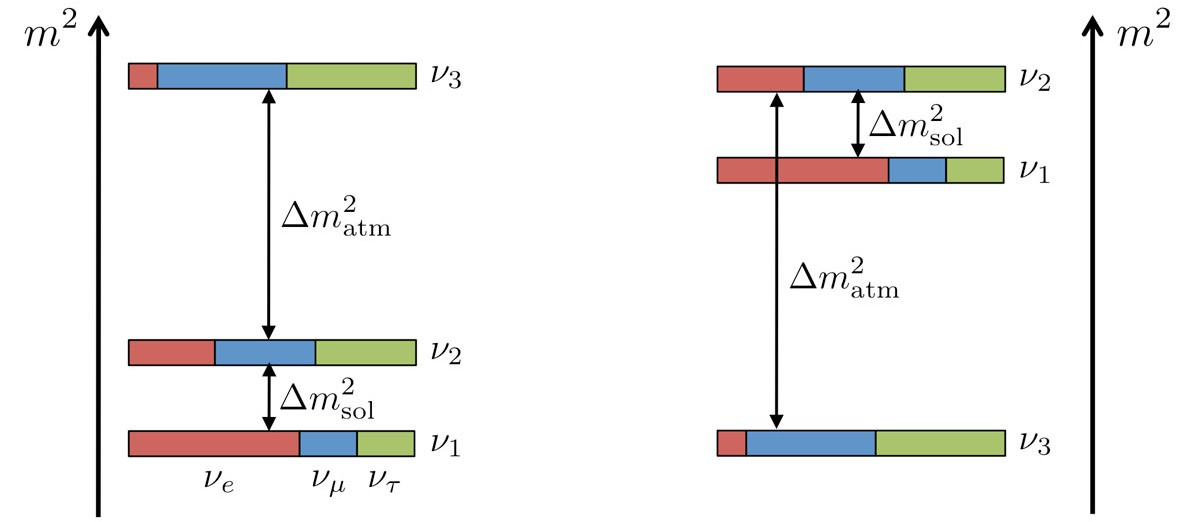
\includegraphics[width = 0.7\textwidth]{figures/mass-hierarchy.jpg}
    \caption{Representation of the two possible mass orderings: normal ordering on the left and inverted ordering on the right.
    The Figure specifies that $\Delta m^2_{21}$ is obtained via solar neutrinos measurements while $\Delta m^2_{32}$ 
    is given by atmospheric neutrinos experiments. Different colours refer to different neutrino flavours: red for the electron flavour, 
    blue for the muon one and green for the tau, respectively. Figure taken from \cite{fermilab-mass-ordering}.}
    \label{fig:mass-ordering}
\end{figure}


\subsection{The Seesaw mechanism}
\label{subsec:seesaw}
Experimental studies confirm that neutrinos do have masses, therefore there must be a corresponding mass term in the Lagrangian. 
Said term can be introduced using the conjugate Higgs field yielding a Dirac mass term after the \ac{SSB} as expressed in Eq. \ref{eq:neutrinos-dirac-masses}
\begin{equation}
    \label{eq:neutrinos-dirac-masses}
    \mathcal{L}_{D} = - m_D (\overline{\nu}_\text{R}\nu_\text{L} + \overline{\nu}_\text{L}\nu_\text{R}) = -\frac{1}{2}m_D (\overline{\nu_\text{L}}\nu_\text{R} + \overline{\nu_\text{R}^c}\nu_\text{L}^c) + h.c.
\end{equation}
where in the second part we used the equivalence of $\overline{\nu_\text{L}}\nu_\text{R} \longleftrightarrow \overline{\nu_\text{R}^c}\nu_\text{L}^c $.
It is clear that if this is the origin of neutrino masses, then \ac{RH}\footnote{Unless otherwise specified right and left refers to chiral states.}
neutrinos -and \ac{LH} antineutrinos as well- must exist. However neutrino masses are much smaller than those of other fermions, either the charged leptons or the quarks for which masses arise in the Higgs mechanism, suggesting that there might be a different phenomenon which generates neutrino masses.

Seeing that \ac{RH} neutrinos and \ac{LH} antineutrinos transform as singlets in the \ac{SM} transformations, any additional term formed by these fields can be added in the the \ac{SM} Lagrangian without breaking its gauge invariance.

While \ac{RH} neutrinos appear as such in the new Lagrangian term, \ac{LH} antineutrinos are defined as the \ac{CP} conjugate fields of \ac{RH} neutrinos as written in Eq. \ref{eq:CPconjugation-righHanded}
\begin{equation}
    \label{eq:CPconjugation-righHanded}
    \psi^c = \hat{C}\hat{P}\psi = i\gamma^2\gamma^0\psi^*.
\end{equation} 
Therefore in the Majorana mass term of Eq. \ref{eq:neutrinos-majorana-masses}, \ac{LH} antineutrinos are written as $\nu_\text{R}^c$ yielding
\begin{equation}
    \label{eq:neutrinos-majorana-masses}
    \mathcal{L}_M = -\frac{1}{2} M \left( \overline{\nu_\text{R}^c} \nu_\text{R} + \overline{\nu_\text{R}} \nu_\text{R}^c \right).
\end{equation}
 

This term clearly respects the local gauge invariance of the \ac{SM}, and consequently it can be added to the \ac{SM} Lagrangian. 
It is now crucial to notice that the Majorana mass term provides a direct coupling between a particle and an antiparticle. 
Thus the corresponding Majorana mass term for the electron would allow $e^+ \leftrightarrow e^-$ transitions, violating charge conservation. 
This problem does not exist for the neutrinos. Nevertheless, seeing that neutrinos are neutral, it is possible that they are their own 
antiparticles, in which case they are referred to as \textit{Majorana neutrinos} and not as \textit{Dirac neutrinos}.

Finally, we can get the general \ac{SM} lagrangian term for neutrino masses including both Eq. \ref{eq:neutrinos-dirac-masses} 
and \ref{eq:neutrinos-majorana-masses} obtaining Eq. \ref{eq:neutrinos-diracANDmajorana-masses}.
\begin{equation}
    \label{eq:neutrinos-diracANDmajorana-masses}
    \mathcal{L}_{DM} = -\frac{1}{2} \left[ m_D \overline{\nu_\text{L}}\nu_\text{R} + m_D \overline{\nu_\text{R}^c}\nu_\text{L}^c + M \overline{\nu_\text{R}^c}\nu_\text{R} \right] + h.c.
\end{equation}
The two different couplings can be represented using Feynman diagrams as depicted in Figure \ref{fig:feynman-massCouplings}.
\begin{figure}[H]
    \centering
    \begin{tikzpicture}[
    thick,
    % Stile per i fermioni (linea continua con freccia a metà)
    fermion/.style={draw=black, postaction={decorate},
        decoration={markings, mark=at position 0.55 with {\arrow{latex}}}},
    % Stile per il campo scalare (linea tratteggiata)
    scalar/.style={draw=black, dashed},
    % Stile per la X
    cross/.style={cross out, draw=black, thick, minimum size=8pt, inner sep=0pt},
    % Stile per il vertice puntiforme
    dot/.style={circle, fill=black, minimum size=4pt, inner sep=0pt}
]

% ---------------- DIAGRAMMA DI DIRAC (Sinistra) ----------------
\coordinate (D) at (0,0);

% Linee entrante e uscente
\draw[fermion] (-1.5, 1.5) node[left] {$\nu_L$} -- (D);
\draw[fermion] (D) -- (1.5, 1.5) node[right] {$\nu_R$};

% Linea tratteggiata (Higgs) con la X finale
\draw[scalar] (D) -- (0, -1.5);
\node[cross] at (0, -1.5) {};

% Vertice centrale con pallino e label
\node[dot, label=right:{$m_D$}] at (D) {};


% ---------------- DIAGRAMMA DI MAJORANA (Destra) ----------------
\coordinate (M) at (6, 0.5); % Spostato a destra e leggermente in alto per allineamento visivo

% Linee (entrambe puntano verso il centro)
\draw[fermion] (4, 0.5) node[left] {$\nu_R$} -- (M);
\draw[fermion] (8, 0.5) node[right] {$\overline{\nu}_L$} -- (M);

% Vertice centrale con la X e label
\node[cross, label=above:{$M$}] at (M) {};

\end{tikzpicture}
    \caption{Feynman diagrams of the two possible mass couplings. On the left the Dirac coupling, associated with $m_D$. On the right the Majorana coupling, associated with $M$.}
    \label{fig:feynman-massCouplings}
\end{figure}

Eq. \ref{eq:neutrinos-diracANDmajorana-masses} can be equivalently rewritten as Eq. \ref{eq:neutrinos-diracANDmajorana-masses-matrix}
\begin{equation}
    \label{eq:neutrinos-diracANDmajorana-masses-matrix}
    \mathcal{L}_{DM} = -\frac{1}{2} \left( \overline{\nu_\text{L}} \quad \overline{\nu_\text{R}^c} \right) \underbrace{\begin{pmatrix} 0 & m_D \\ m_D & M \end{pmatrix}}_{\mathbf{M}} \begin{pmatrix} \nu_\text{L}^c \\ \nu_\text{R} \end{pmatrix} + \text{h.c.}
\end{equation}

where we identified the mass matrix $\mathbf{M}$, that can be diagonalised in order to define the physical states. 
Through the characteristic equation$\text{det}(\mathbf{M} - \lambda \mathbb{1})$ that yields $\lambda^2 - M\lambda - m_D^2 = 0$, 
one get the masses of the physical neutrinos that are 
\begin{equation*}
    m_{\pm} = \lambda_{\pm} = \frac{M \pm \sqrt{M^2 + 4m_D^2}}{2} = \frac{M \pm M\sqrt{1 + 4m_D^2/M^2}}{2}.
\end{equation*}
Furthermore, taking the Majorana mass $M$ much greater than the Dirac mass $m$, 
i.e. $M \gg m_D$\footnote{Dirac mass is assumed to be of the same order of the mass of the other fermions ($\mathcal{O}(1~\text{GeV})$) 
while the Majorana mass term is thought to be very large ($\mathcal{O}(10^{11}~\text{GeV})$) in order to get $m_\nu \sim 0.01$~eV}, 
the two possible masses reduce to 
\begin{equation*}
    m_{\pm} \approx \frac{1}{2}M \pm \frac{1}{2}\left( M + \frac{2m_D^2}{M} \right)
\end{equation*}
giving a light neutrino state ($\nu$) and an heavy neutrino state ($N$) with the masses reported in Eq. \ref{eq:final-nu-masses}
\begin{equation}
    \label{eq:final-nu-masses}
    |m_{\nu}| \approx \frac{m_D^2}{M} \quad \text{and} \quad m_N \approx M.
\end{equation} 
Therefore, if we go back to Eq. \ref{eq:neutrinos-diracANDmajorana-masses-matrix} we can rewrite $\nu$ and $N$ as a function of
$\overline{\nu_\text{L}}$, $\overline{\nu_\text{L}^c}$, $\overline{\nu_\text{R}}$ and $\overline{\nu_\text{R}^c}$ as shown in Eq. \ref{eq:neutrinos-revisited}
\begin{equation}
    \label{eq:neutrinos-revisited}
    \nu = \cos\theta (\nu_\text{L} + \nu_\text{L}^c) - \sin\theta (\nu_\text{R} + \nu_\text{R}^c) \quad \text{and} \quad N = \cos\theta (\nu_\text{R} + \nu_\text{R}^c) + \sin\theta (\nu_\text{L} + \nu_\text{L}^c)
\end{equation}
where the mixing angle $\theta$ is determined by the ratio of the Dirac and Majorana masses, with $\theta = \frac{m_D}{M}$. 
Since the Majorana mass scale $M$ is assumed to be enormous compared to the Dirac mass, this ratio is extremely small. 
Consequently, $\theta$ tends to zero and this allows us to apply the small-angle approximations for the trigonometric functions such that
$\tan\theta \sim \theta \sim \frac{m_D}{M}~$ and consequently one gets $~\cos\theta \sim 1~$ and $~\sin\theta \sim \theta = \frac{m_D}{M}~$.\\
This consideration yields
\begin{equation*}
    \nu \approx (\nu_\text{L} + \nu_\text{L}^c) - \frac{m_D}{M}(\nu_\text{R} + \nu_\text{R}^c) ~ \text{and} ~ N \approx (\nu_\text{R} + \nu_\text{R}^c) + \frac{m_D}{M}(\nu_\text{L} + \nu_\text{L}^c).
\end{equation*}
It is now evident that the light-neutrino state is almost entirely \ac{LH} while the heavy-neutrino one is almost entirely \ac{RH}. 
Therefore the latter is not participating in the weak \ac{CC} interactions neither in the weak \ac{NC} interactions of the \ac{SM}.

The process described so far, set against the Higgs mechanism for mass, is known as \textit{seesaw mechanism}.\\
This is just an hypothesis, but it would be more grounded if neutrinos were shown to be Majorana particles.\\
The latter could be done if we would observe the neutrinoless double $\beta$-decay that will be discussed further in this work in Section \ref{subsec:0nubetabeta}.

\section{Beta decay and double beta decay}
Beta decay is a nuclear transition in which a nucleus $(Z, A)$ converts into an isobar $(Z \pm 1, A)$ through the weak interaction, with the emission of an electron or positron and the corresponding (anti)neutrino, as anticipated in Section~\ref{sec:nuIntro}. The single-beta decay process can be written as
\begin{equation}
    \label{eq:single-beta-decay}
    (Z, A) \longrightarrow (Z+1, A) + e^- + \overline{\nu}_e \qquad \text{or} \qquad 
    (Z, A) \longrightarrow (Z-1, A) + e^+ + \nu_e,
\end{equation}
depending on whether a neutron ($\beta^-$) or a proton ($\beta^+$) undergoes the weak transition. Enrico Fermi described this process in 1934 by introducing a point-like, four-fermion contact interaction Hamiltonian
\begin{equation}
    H_F = G_F \left( \overline{\psi}_p \gamma^\mu \psi_n \right)\left( \overline{\psi}_e \gamma_\mu \psi_\nu \right) + \text{h.c.}
\end{equation} 
with $G_F$ the Fermi coupling constant, later reinterpreted within the \ac{SM} as the low-energy, effective limit of the \ac{CC} interaction (Eq. \ref{eq:SM-neutrino-lagrangian}) where a virtual $W$ boson mediates, at the quark level, the $d \to u$ or $u \to d$ transitions. The process is allowed whenever it is energetically favourable, i.e. whenever the mass difference between the mother and daughter nuclei is large enough to compensate for the $Q$-value of the reaction, and it is precisely this energy balance, together with nuclear pairing effects, that determines which nuclei undergo ordinary $\beta$ decay and which ones are instead only accessible through the second-order process of double-$\beta$ decay, discussed further in this Section.

\subsection{Two-neutrino double beta decay (\texorpdfstring{$2\nu\boldsymbol{\beta}\boldsymbol{\beta}$}{2vbb})}
\label{subsec:2nubetabeta}

Two-neutrino double beta decay ($2\nu\beta\beta$) is a second-order weak interaction process in which a nucleus $(Z, A)$ decays directly into its isobar $(Z+2, A)$ with the simultaneous emission of two electrons and two electron antineutrinos. First proposed in 1935 by Maria Goeppert-Mayer \cite{firstDoubleBeta}, this decay mode perfectly conserves the lepton number and is fully accommodated within the \ac{SM}. The transition is described by the reaction:
\begin{equation}
    \label{eq:2nubetabeta}
    (Z, A) \longrightarrow (Z+2, A) + 2e^- + 2\overline{\nu}_e.
\end{equation}
At the microscopic level, the process occurs through two simultaneous, virtual single-$\beta$ transitions, as illustrated by the two weak vertices in the Feynman diagram of Figure \ref{fig:2nu_feynman}.

\begin{figure}[H]
    \centering
    \begin{center}
\begin{tikzpicture}[
    thick,
    % Stile per le linee dei fermioni (linea con freccia a metà)
    fermion/.style={draw=black, postaction={decorate},
        decoration={markings, mark=at position 0.55 with {\arrow{latex}}}},
    % Stile per i bosoni W (linea ondulata)
    boson/.style={draw=black, decorate,
        decoration={snake, amplitude=1mm, segment length=3.5mm}},
    % Stile per i vertici dei nucleoni (i cerchi grigi)
    blob/.style={circle, draw=black, fill=gray!30, minimum size=6mm, inner sep=0pt}
]

% ---------------- NUCLEONE SUPERIORE ----------------
% Frecce esterne n e p
\draw[fermion] (-4.5, 2) node[left, font=\Large] {n} -- (-3, 2);
\draw[fermion] (3, 2) -- (4.5, 2) node[right, font=\Large] {p};

% Le 3 linee dei quark all'interno (tra i due blob)
\draw[fermion] (-3, 2.15) -- (3, 2.15);
\draw[fermion] (-3, 2.0) -- (3, 2.0);
\draw[fermion] (-3, 1.85) -- (3, 1.85);

% Bosone W- 
\draw[boson] (0, 1.85) -- (1.5, 0.8);
\node[font=\Large] at (0.4, 1.2) {$W^-$};

% Elettrone e antineutrino 
% (Nota: la linea del neutrino è disegnata da destra a sinistra per invertire la freccia)
\draw[fermion] (1.5, 0.8) -- (3.5, 1.3) node[right, font=\Large] {$e^-$};
\draw[fermion] (3.5, 0.3) node[right, font=\Large] {$\overline{\nu}_e$} -- (1.5, 0.8);


% ---------------- NUCLEONE INFERIORE ----------------
% Frecce esterne n e p
\draw[fermion] (-4.5, -2) node[left, font=\Large] {n} -- (-3, -2);
\draw[fermion] (3, -2) -- (4.5, -2) node[right, font=\Large] {p};

% Le 3 linee dei quark all'interno (tra i due blob)
\draw[fermion] (-3, -1.85) -- (3, -1.85);
\draw[fermion] (-3, -2.0) -- (3, -2.0);
\draw[fermion] (-3, -2.15) -- (3, -2.15);

% Bosone W- 
\draw[boson] (0, -1.85) -- (1.5, -0.8);
\node[font=\Large] at (0.4, -1.2) {$W^-$};

% Elettrone e antineutrino
\draw[fermion] (1.5, -0.8) -- (3.5, -0.3) node[right, font=\Large] {$e^-$};
\draw[fermion] (3.5, -1.3) node[right, font=\Large] {$\overline{\nu}_e$} -- (1.5, -0.8);


% --- DISEGNO I BLOB ---
% (Disegnati per ultimi così coprono perfettamente le estremità delle linee)
\node[blob] at (-3, 2) {};
\node[blob] at (3, 2) {};
\node[blob] at (-3, -2) {};
\node[blob] at (3, -2) {};

\end{tikzpicture}
\end{center}
    \caption{Feynman diagram of $2\nu\beta\beta$. The process proceeds via the exchange of two virtual $W^-$ bosons, resulting in the simultaneous emission of two electrons and two electron antineutrinos.}
    \label{fig:2nu_feynman}
\end{figure}

\begin{wrapfigure}{r}{0.52\textwidth}%[H]
    \centering
    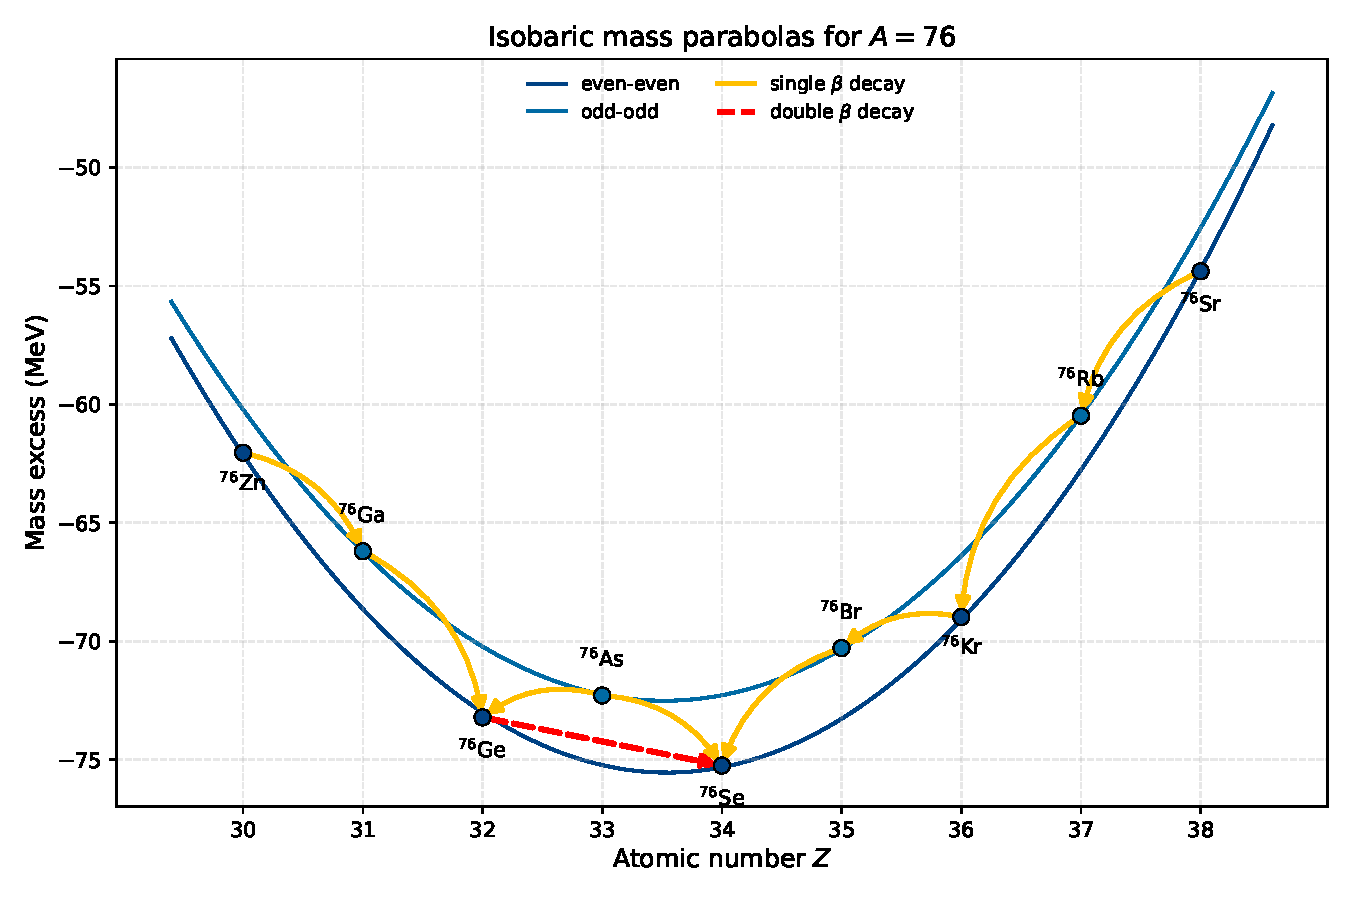
\includegraphics[width=\linewidth]{figures/mass_parabola_A76.pdf}
    \caption{Mass parabolas for $A=76$ isobars. A detailed description is given in the text. Custom plot with data taken from \cite{AME2020-masses} and \cite{Ge76-Qvalue}.}
    \label{fig:doublebeta-parabola}
\end{wrapfigure}
For a nucleus to undergo such a rare decay, the standard single-$\beta$ decay to the intermediate isobar $(Z+1, A)$ must be energetically forbidden or heavily suppressed. This kinematic condition naturally arises in even-even nuclei due to the nuclear pairing interaction, which binds them more tightly than their odd-odd neighbours. As a consequence, while the direct transition $(Z, A) \to (Z+1, A)$ is blocked, the target state $(Z+2, A)$ still sits at a lower energy level, effectively opening the double-$\beta$ channel. 
This energy landscape is visualised using mass parabolas, as shown in Figure \ref{fig:doublebeta-parabola} for the case of ${}^{76}\text{Ge}$, where the even-even and odd-odd mass parabolas are shown with a continuous and dashed line, respectively. The double-beta transition of ${}^{76}\text{Ge}$ is highlighted in red, while the yellow lines represent ordinary single-$\beta$ decays. The intermediate odd-odd state acts as a virtual state in the quantum mechanical transition and is never physically populated.

Because $2\nu\beta\beta$ is a second-order process in the weak coupling, its decay rate is massively suppressed compared to ordinary $\beta$ decay, resulting in extremely long half-lives of the order of $T_{1/2}^{2\nu} \sim 10^{19}$--$10^{24}$~years, depending on the isotope.

Unlike the neutrinoless mode, $2\nu\beta\beta$ does not require any new physics beyond the \ac{SM} and has been experimentally observed in about different even-even isotopes. Nuclei such as ${}^{76}\text{Ge}$ are of particular relevance in modern physics, as they also represent the most promising candidates in the search for neutrinoless double beta decay, a process that violates lepton number by two units and is discussed in detail in Section~\ref{subsec:0nubetabeta}.

\subsection{Neutrinoless double beta decay (\texorpdfstring{$0\nu\boldsymbol{\beta}\boldsymbol{\beta}$}{0vbb})}
\label{subsec:0nubetabeta}

The most sensitive probe to determine whether neutrinos are Dirac or Majorana particles -as introduced in Section \ref{subsec:seesaw}- is the neutrinoless double $\beta$-decay ($0\nu\beta\beta$), detailed in Eq. \ref{eq:0nu-beta-beta} and Figure \ref{fig:0nubetabeta-diagram}:
\begin{equation}
    \label{eq:0nu-beta-beta}
    (Z, A) \longrightarrow (Z+2, A) + 2e^-
\end{equation} 

\begin{figure}[H]
    \centering
    \begin{center}
\begin{tikzpicture}[
    thick,
    % Stile per le linee dei fermioni (linea con freccia a metà)
    fermion/.style={draw=black, postaction={decorate},
        decoration={markings, mark=at position 0.55 with {\arrow{latex}}}},
    % Stile per i bosoni W (linea ondulata)
    boson/.style={draw=black, decorate,
        decoration={snake, amplitude=1mm, segment length=3.5mm}},
    % Stile per la massa di Majorana (la X al centro)
    cross/.style={cross out, draw=black, thick, minimum size=6pt, inner sep=0pt},
    % Stile per i vertici dei nucleoni (i cerchi grigi)
    blob/.style={circle, draw=black, fill=gray!30, minimum size=6mm, inner sep=0pt}
]

% ---------------- NUCLEONE SUPERIORE ----------------
% Frecce esterne n e p
\draw[fermion] (-4, 2) node[left] {n} -- (-2.5, 2);
\draw[fermion] (2.5, 2) -- (4, 2) node[right] {p};

% Le 3 linee dei quark all'interno
\draw[fermion] (-2.5, 2.15) -- (2.5, 2.15);
\draw[fermion] (-2.5, 2.0) -- (2.5, 2.0);
\draw[fermion] (-2.5, 1.85) -- (2.5, 1.85);


% ---------------- NUCLEONE INFERIORE ----------------
% Frecce esterne n e p
\draw[fermion] (-4, -2) node[left] {n} -- (-2.5, -2);
\draw[fermion] (2.5, -2) -- (4, -2) node[right] {p};

% Le 3 linee dei quark all'interno
\draw[fermion] (-2.5, -1.85) -- (2.5, -1.85);
\draw[fermion] (-2.5, -2.0) -- (2.5, -2.0);
\draw[fermion] (-2.5, -2.15) -- (2.5, -2.15);


% --- DISEGNO I BLOB ---
% (Disegnati per ultimi così coprono perfettamente le estremità delle linee)
\node[blob] at (-2.5, 2) {};
\node[blob] at (2.5, 2) {};
\node[blob] at (-2.5, -2) {};
\node[blob] at (2.5, -2) {};


% ---------------- SCAMBIO INTERNO (W, neutrini ed elettroni) ----------------
% Bosoni W (partono dalla linea del quark più vicina al centro)
\draw[boson] (-0.5, 1.85) -- (0.5, 0.7);
\draw[boson] (-0.5, -1.85) -- (0.5, -0.7);

% Linea del neutrino di Majorana (dritta, senza freccia, con la X)
\draw (0.5, 0.7) -- (0.5, -0.7);
\node[cross, label=right:{$\nu_M$}] at (0.5, 0) {};

% Elettroni uscenti
\draw[fermion] (0.5, 0.7) -- (2.5, 1.2) node[right] {e$^-$};
\draw[fermion] (0.5, -0.7) -- (2.5, -1.2) node[right] {e$^-$};

\end{tikzpicture}
\end{center}
    \caption{Feynman diagram for neutrinoless double $\beta$-decay. The Majorana coupling of the neutrino with its own antineutrino (see Figure \ref{fig:feynman-massCouplings}) is shown.}
    \label{fig:0nubetabeta-diagram}
\end{figure}

\begin{wrapfigure}{l}{0.52\textwidth}%[H]
    \centering
    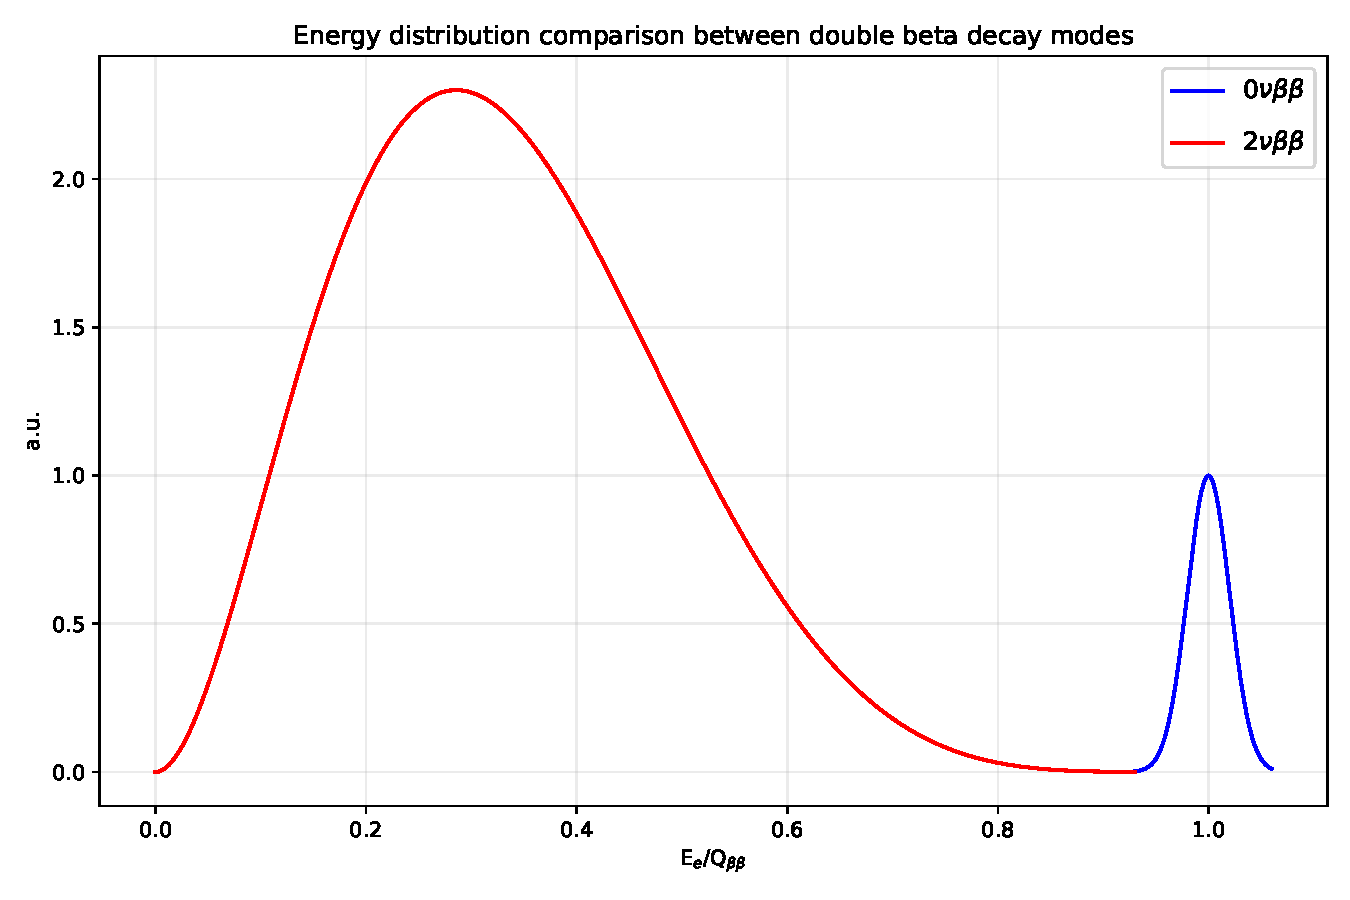
\includegraphics[width=\linewidth]{figures/0nu_vs_2nu.pdf}
    \caption{Schematic representation of the energy distribution for the products in $2\nu\beta\beta$ and $0\nu\beta\beta$ decay modes. The description is given in the text.}
    \label{fig:Qvalue-2nu0nu}
\end{wrapfigure}
From an experimental point of view, a $0\nu\beta\beta$ process can be distinguished from the more common $2\nu\beta\beta$ decay by analyzing the electron energy spectra of the two emitted electrons. Specifically, in $0\nu\beta\beta$ decay, the electrons are produced with energies $E_{e, 1}$ and $E_{e, 2}$ that satisfies
\begin{equation*}
    E_{e, 1} + E_{e, 2} + E_{\text{nuc}} = Q_{\beta\beta} = \frac{1}{2} [M(Z, A) - M(Z+2, A)] 
\end{equation*}
where $M(Z, A)$ and $M(Z+2, A)$ represent the masses of the parent and daughter nuclei, respectively. Moreover, the energy of the recoiling nucleus being negligible, the sum of the electron energies is equal to the $Q$-value of the transition, i.e. $E_{e, 1} + E_{e, 2} = Q_{\beta\beta}$. Conversely, for standard $2\nu\beta\beta$ decay, the combined electron energy spectrum is continuous, with very few events occurring near the endpoint $\frac{1}{2}Q$. Fig. \ref{fig:Qvalue-2nu0nu} shows said continuous spectrum in red for the $2\nu\beta\beta$ process and the monoenergetic one around the $Q$-value for $0\nu\beta\beta$ in blue.

If neutrinos are indeed Majorana particles, the standard mechanism for $0\nu\beta\beta$ decay is mediated by the exchange of a light Majorana neutrino. The decay rate, usually expressed in terms of the half-life $T_{1/2}^{0\nu}$, is given by:
\begin{equation}
    \label{eq:half-life_0nubb}
    (T_{1/2}^{0\nu})^{-1} = G_{0\nu}(Q, Z) \left| \mathcal{M}_{0\nu} \right|^2 \left( \frac{m_{\beta\beta}}{m_e} \right)^2
\end{equation}
where $G_{0\nu}(Q, Z)$ is the phase space factor (which depends on the Q-value and the atomic number $Z$), $\mathcal{M}_{0\nu}$ is the nuclear matrix element, $m_e$ is the electron mass, and $m_{\beta\beta} = \sum_{i=1}^{3} U_{ei}^2 m_{\nu i}$ denotes the effective Majorana mass, which depends on both the PMNS matrix elements and the neutrino mass eigenvalues. Consequently, the decay rate is directly sensitive to the \ac{NMO}.

Experimentally, observing $0\nu\beta\beta$ decay requires identifying a tiny, mono-energetic signal at $Q_{\beta\beta}$, so the coice of the best isotope to search for such rare decay is the first thing to face, since it involves background suppression and energy resolution considerations but also the limited time for which an experiment can be used. These result in a series of criteria to be considered in choosing the suitable isotope, which restrict the choice to elemtns with high isotopic abundance, a good compatibility with detection tecniques and a sufficiently high $Q$-value above $\sim2400$~keV in order to reduce the $\gamma$-induced background\footnote{Specifically, the end-point of natural gamma radioactivity is set to the $2615$~keV line of ~${}^{208}$Tl.} or even at higher energies, i.e. above $3270$~keV, to reduce the contaminations from $\beta$ deccays of the ~${}^{238}$U chain. \cite{review-0nu-2015}

Thus, the commonly studied isotopes are the ones listed in Table \ref{tab:istopes-for-0nu} together with their isotopic abundance and $Q_{\beta\beta}$ values. ${}^{76}$Ge represents an exception among the others because $Q_{\beta\beta} = 2039$~keV: this is in principle a limitation in terms of background reduction, since natural $\gamma$ radioactivity is highly present in that energy range, but it nevertheless one of the most notable isotopes because of its powerful detection tecniques. 

\begin{table}[H]
    \centering
    \begin{tabular}{lcc}
        \toprule
        Isotope & Isotopic abundance (\%) & $Q_{\beta\beta}$ [keV] \\
        \midrule
        ${}^{48}\text{Ca}$  & 0.187 & 4263 \\
        \rowcolor{greyblue}
        ${}^{76}\text{Ge}$  & 7.8   & 2039 \\
        ${}^{82}\text{Se}$  & 9.2   & 2998 \\
        ${}^{96}\text{Zr}$  & 2.8   & 3348 \\
        ${}^{100}\text{Mo}$ & 9.6   & 3035 \\
        ${}^{116}\text{Cd}$ & 7.6   & 2813 \\
        ${}^{130}\text{Te}$ & 34.08 & 2527 \\
        ${}^{136}\text{Xe}$ & 8.9   & 2459 \\
        ${}^{150}\text{Nd}$ & 5.6   & 3371 \\
        \bottomrule
    \end{tabular}
    \caption{Candidate isotopes for $0\nu\beta\beta$ search: isotopic abundance and $Q_{\beta\beta}$ value. Data are taken from \cite{review-0nu-2015}.}
    \label{tab:isotopes-for-0nu}
\end{table}

The decay half-life of a $0\nu\beta\beta$ event, if detected, can be evaluated as 
\begin{equation}
    \label{eq:half-life_0nubb}
    t^{1/2} = \ln(2) \cdot T \cdot \varepsilon \cdot \frac{N_{\beta\beta}}{N_\text{peak}}
\end{equation}
where $T$ is the measuring time, $\varepsilon$ is the detection efficiency, $N_{\beta\beta}$ is the number of $\beta\beta$ decaying nuclei under observation and $N_\text{peak}$ is the number of observed decays in the region of interest. If no peak is detected, the sensitivity of a given experiment is expressed in terms of a detector \textit{factor of merit} $S^{0\nu}$, i.e. the process half-life corresponding to the maximum signal that could be hidden by the background fluctuations $n_{B}$. From Eq.~\ref{eq:half-life_0nubb}, the sensitivity can be written as
\begin{equation}
    \label{eq:sensitivity-0nu}
    \begin{aligned}
        S^{0\nu} &= \ln 2 \cdot T \cdot \varepsilon \cdot \frac{n_{\beta\beta}}{n_\sigma \cdot n_B} \\
                 &= \ln 2 \cdot \varepsilon \cdot \frac{1}{n_\sigma} \cdot \frac{x\,\eta\,N_A}{\mathcal{M}_A} \cdot \sqrt{\frac{M \cdot T}{B \cdot \Delta E}},
    \end{aligned}
\end{equation}
where $\varepsilon$ is the detection efficiency, $n_\sigma$ the confidence level in units of standard deviations, and $n_{\beta\beta}$ and $n_B$ the numbers of signal and background events \cite{review-0nu-2015}. The exposure $M \cdot T$\footnote{$\text{Exposure [kg yr]} = \text{Detector mass [kg]} \cdot \text{Livetime [yr]}$} is the product of detector mass and measuring time, $B$ is the background level per unit mass, energy and time, and $\Delta$ is the energy resolution (FWHM) at $Q_{\beta\beta}$. Finally, $x$ is the stoichiometric multiplicity of the candidate element, $\eta$ its isotopic abundance, $N_A$ Avogadro's number and $\mathcal{M}_A$ the molar mass of the compound.

This formula dictates the design of modern experiments: to maximize sensitivity, one must increase the exposure while minimizing both the background levels and the energy resolution. Specifically, a poor energy resolution causes the continuous tail of the standard $2\nu\beta\beta$ decay to smear into the $0\nu\beta\beta$ region of interest, creating an irreducible background.

\newpage
\section{Experiments currently searching for \texorpdfstring{$0\nu\boldsymbol{\beta}\boldsymbol{\beta}$}{0nu beta beta} decay}
\label{sec:0nubb-experiments}
The experimental approach to $0\nu\beta\beta$ searching is based on the development of a proper detection tecnique able to balance good energy resolution, very low background and large isotope mass. Up to now, experiments in this field rely on two different tecnicques: detectors based on a calorimetric tecnique, for which the source is embedded inside the detector volume itself, and detectors exploiting an external source \cite{review-0nu-2015}. 

The best limits obtained so far for each candidate isotope are reported in Table~\ref{tab:0nubb-limits} \cite{PDG:2026}, while the experiments currently running or planned, together with their expected sensitivities, are summarised in Fig.~\ref{fig:experiments-and-sensitivities-0nubb}, where experiments marked in green exploit ${}^{100}$Mo, those in yellow use ${}^{136}$Xe, the blue ones employ ${}^{130}$Te, SuperNEMO is the only one using ${}^{82}$Se and finally red experiments exploit ${}^{76}$Ge.

\begin{table}[H]
    \centering
    \begin{tabular}{llc}
        \toprule
        Isotope & Experiment & $T_{1/2}^{0\nu}$ limit [yr] \\
        \midrule
        ${}^{48}\text{Ca}$  & CaF$_2$ scintillators     & $> 5.8 \times 10^{22}$ \\
        ${}^{76}\text{Ge}$  & GERDA + MJD + LEGEND-200  & $> 1.9 \times 10^{26}$ \\
        ${}^{82}\text{Se}$  & CUPID-0                   & $> 4.6 \times 10^{24}$ \\
        ${}^{96}\text{Zr}$  & NEMO-3                    & $> 9.2 \times 10^{21}$ \\
        ${}^{100}\text{Mo}$ & AMoRE-I                   & $> 2.9 \times 10^{24}$ \\
        ${}^{116}\text{Cd}$ & AURORA                    & $> 2.2 \times 10^{23}$ \\
        ${}^{130}\text{Te}$ & CUORE                     & $> 3.5 \times 10^{25}$ \\
        ${}^{136}\text{Xe}$ & KamLAND-Zen               & $> 3.8 \times 10^{26}$ \\
        ${}^{150}\text{Nd}$ & NEMO-3                    & $> 2.0 \times 10^{22}$ \\
        \bottomrule
    \end{tabular}
    \caption{Best current lower limits (90\% CL) on the $0\nu\beta\beta$ half-life for each candidate isotope \cite{PDG:2026}.}
    \label{tab:0nubb-limits}
\end{table}

\begin{figure}[H]
    \centering
    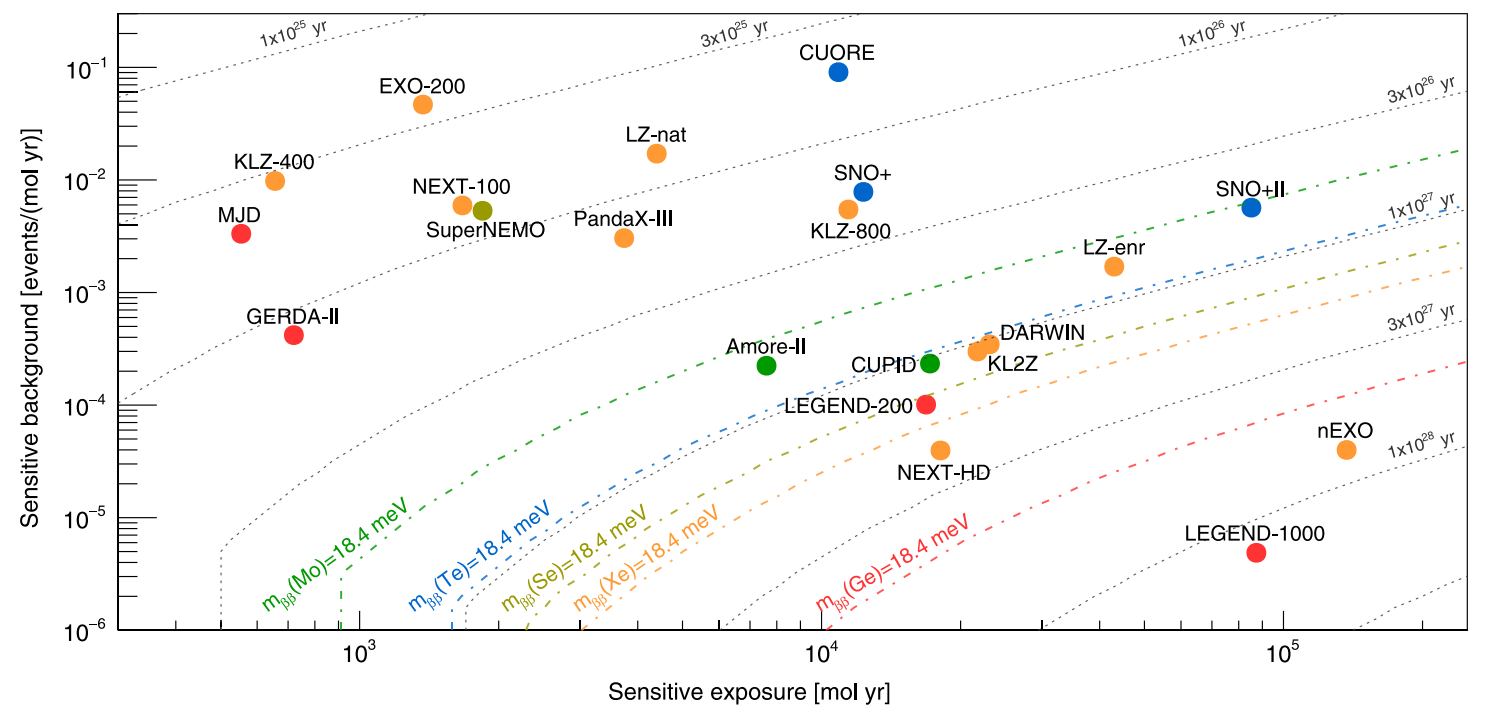
\includegraphics[width=\textwidth]{figures/experiments_and_sensitivities.png}
    \caption{Overview of the experiments searching for $0\nu\beta\beta$ decays with related sensitive exposures and backgrounds. Plot taken from \cite{plot-esperiments_and_exposures}.}
    \label{fig:experiments-and-sensitivities-0nubb}
\end{figure}